\section{Methods} \label{sec:methods}

In this section, we describe the primary two algorithmic components for our on-device simulation:
\begin{enumerate}
\item the asynchronous compute-communicate cycle used to instantiate an island model evolutionary process across the WSE engine, and
\item the lightweight hereditary stratigraphy element used to annotate virtual genomes and facilitate robust post-hoc phylogenetic reconstruction.
\end{enumerate}

\subsection{Asynchronous Island-model Evolutionary Computation}

\begin{wrapfigure}{r}{0.5\textwidth}
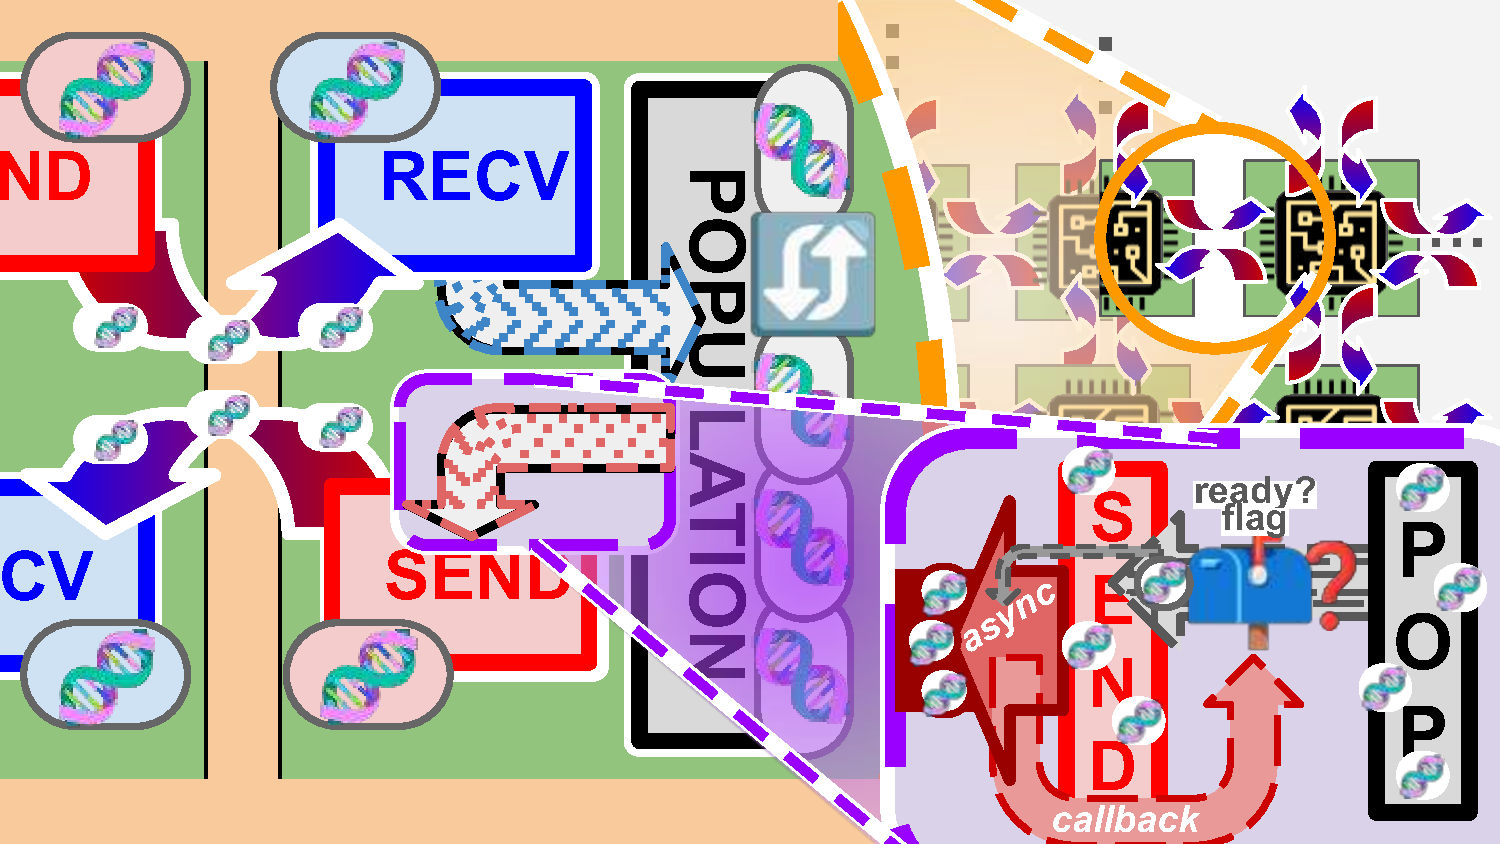
\includegraphics[width=\linewidth]{img/async-ga-schematic.pdf}
\centering
\caption{Schematic overview of asynchronous island model evolutionary algorithm.}
\label{fig:async-ga-schematic}
\end{wrapfigure}

We apply an island-model genetic algorithm to instantiate an evolutionary process spanning PEs.
Island-model approaches are common in applications of parallel and distributed computing to evolutionary computation \citep{bennett1999building}.
Under this model, each processor element (PE) hosts an independent population.
Migration between PEs stitches island populations together into a common gene pool.

Core kernel activity proceeds via an update cycle performed on each PE, which comprises several steps.
Figure \ref{fig:async-ga-schematic} provides a schematic overview.

The first step of this update loop is to handle migration, depicted as blue-red arrows in Figure \ref{fig:async-ga-schematic}.
We adopt a fully asynchronous approach to migration between neighboring PEs.
Evolutionary processes tend to occur in asynchronous manner with arbitrary factors influencing things, so this is a reasonable relaxation to make.

Each PE maintains independent immigration buffers and emigration buffers dedicated to each cardinal neighbor, depicted in blue and red, respectively, in Figure \ref{fig:async-ga-schematic}.
On simulation startup, an asynchronous DSD receive operation is opened to accept genomes from neighboring PEs into the appropriate immigration buffer.
At startup, additionally, the emigration buffer is populated with one or more genomes copied the population.
Then, an asynchronous send request is opened to dispatch wavelets containing genome data from the emigration buffer to the neighbor.
Both operations register an on-completion callback to set a ``send complete'' or ``receive complete'' flag variable associated with their corresponding buffer.

Each update cycle, the main update loop tests all ``send complete'' and ``receive complete'' flags.
For each immigration flag that is set, corresponding received genomes are written into the main population buffer, replacing randomly-chosen population members.
Then, the flag is reset a new receive request is initiated.
Likewise, for each emigration flag set, corresponding send buffers are re-populated with randomly sampled genomes from the main population buffer.
Corresponding flags are then reset and new send requests initiated.
The bottom right corner of Figure \ref{fig:async-ga-schematic} summarizes this process.

The remainder of the main update loop handles evolutionary operations within the scope of the executing PE.
Each genome within the population is evaluated to produce a floating point fitness value.
Modular implementation ensures evaluation criteria can be chosen appropriate for underlying experimental objectives.
For the purposes this project, we will use a trivial fitness function that explicitly models additive accumulation of beneficial/deleterious mutations as a floating point value within each genome.

After evaluation, tournament selection is applied.
Each slot in the next generation is populated with a genome exhibiting maximal fitness among $n$ randomly sampled individuals, ties broken randomly.

Finally, a mutational operator is applied across all genomes in the next population.
As with evaluation criteria, modular implementation allows mutation operations to be defined based on experimental objectives.
Here, we use a simple Gaussian mutation on each genome's stored fitness value.
At this point, hereditary stratigraphy annotations --- discussed next --- are updated to reflect an elapsed generation.

The process then repeats, with self-activating wavelet dispatched to execute the next cycle of the main update loop.

Kernel source code implementing described procedures can be viewed at \url{https://hopth.ru/cl}.
Our implementation is defined modularity with respect to genome size, layout, mutational operator, and fitness evaluation criteria, allowing for direct re-use of produced software for follow-on evolution experiments on WSE hardware.

% A key question will be the extent to which intentionally desynchronizing affects performance, stability, and computation quality.

\subsection{Distributed Phylogenetic Tracking}

Our approach to analysis of evolutionary history for wafer-scale simulation draws inspiration from the inference-based paradigm used to characterize history in natural systems.
This approach is fully-distributed, with ancestry information contained within genomes themselves rather than in any external tracking mechanism.
Just as mutational drift encodes ancestry information in DNA genomes, the inference-based paradigm requires only local updates to individual genomes at runtime as generations elapse.

Recent work introducing \textit{hereditary stratigraphy} (HStrat) methodology has explored how best to organize genetic material to maximize reconstruction quality and minimize memory footprint \citep{moreno2022hstrat, moreno2022hereditary}.
Proposed work bundles HStrat material with underlying agent genomes as an instrumentative ornament, entirely neutral with respect to agent traits or fitness.

The hereditary stratigraphy algorithm associates each generation along individual lineages with an identifying ``fingerprint'' value.
Each time a generation elapses, all offspring generate a new identifier value.
Within each offspring, generated identifiers append to an inherited running chronological record of fingerprint values.
To prevent $\mathcal{O}(n)$ space complexity as generations elapse, not all fingerprints can be kept.
Instead, excess fingerprints are pruned away according to a deterministic programme that ensures retention of fingerprint values from checkpoint generations spaced across evolutionary history.

% \begin{figure}[htbp]
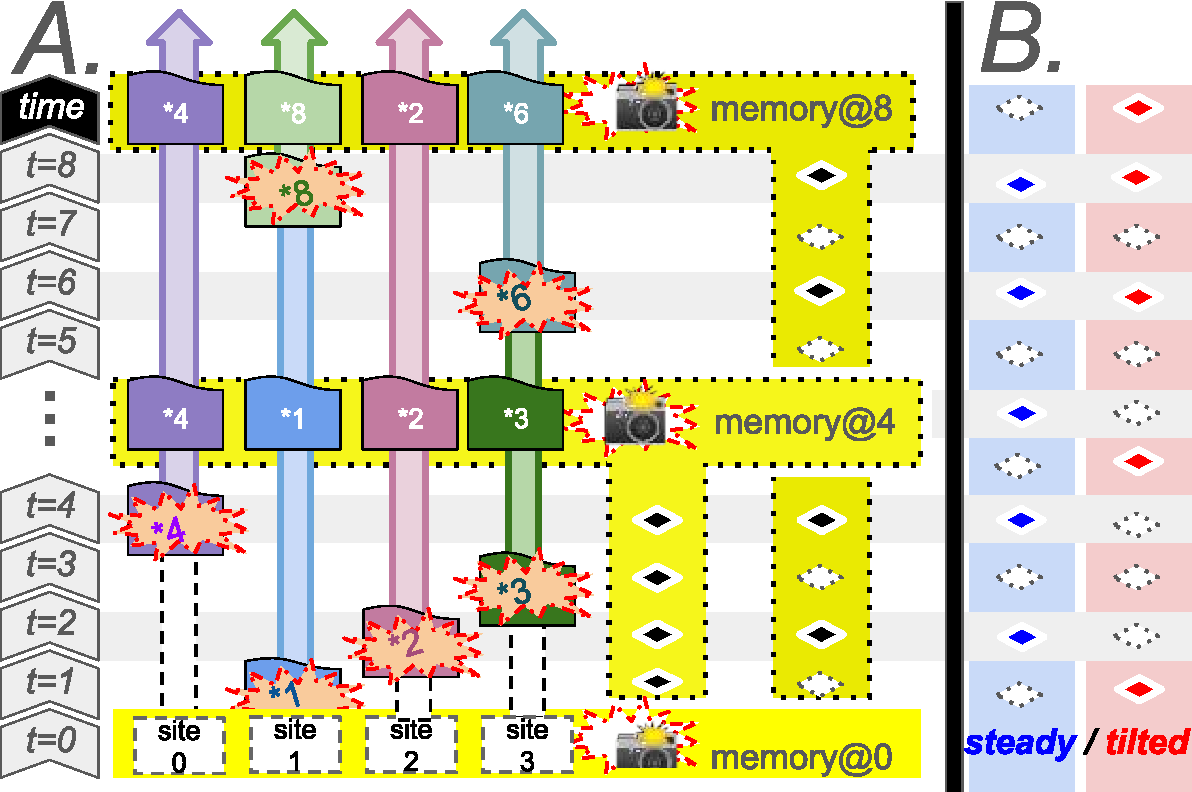
\includegraphics[width=4in]{img/hsurf-schematic.pdf}
\caption{Panel A shows update sequence on a four-site HStrat curation space-time memory under steady policy. Panel B contrasts steady policy with tilted policy, which prioritizes recent data. }
\label{fig:hsurf-schematic}
\end{figure}

Limitations of the Cerebras WSE environment required significant elaboration of hereditary stratigraphy algorithms to minimize memory use, avoid complex data structures with dynamically allocated memory, and minimize iterative computation.
We use a constant-time indexing scheme that maps each lineage's fingerprint stream onto a fixed-width memory buffer such that eviction of existing fingerprint values by new placements maintains a temporally-representative sampling over elapsed time (Figure \ref{fig:hsurf-schematic}a), either evenly (``steady'') or recency-biased (``tilted'') (Figure \ref{fig:hsurf-schematic}b).
We call this approach ``surface''-based to distinguish it from earlier hereditary stratigraphy methods.
Time stamps can be positionally inferred and thus do not need to be stored --- a several-fold savings that enables fingerprint values to be shrunk down and packed together.
Single-bit checkpoints have been shown to produce good quality phylogenies using only 96 bits per genome \citep{moreno2023toward}.
The semantic structure of HStrat annotations streamlines \textit{post hoc} phylogenetic reconstruction, which essentially boils down to a simple trie-building procedure
\citep{moreno2024analysis}.
